\section{Arquitectura}
En esta sección mostraremos los diagramas (\textbf{vista C\&C}) desarrollados para la arquitectura del sistema. Por razones de claridad y espacio, se omitió en el diagrama el detalle de los puertos y roles en los componentes y conectores.

Consideramos nuestra arquitectura con un estilo predominantemente Cliente-Servidor, donde el Servidor es nuestro sistema, distribuido en distintas máquinas (\textit{nodos}) a través del mundo, mientras que el Cliente es el navegador web que se encuentra en el dispositivo que utiliza el usuario.

\subsection{Paneo General}
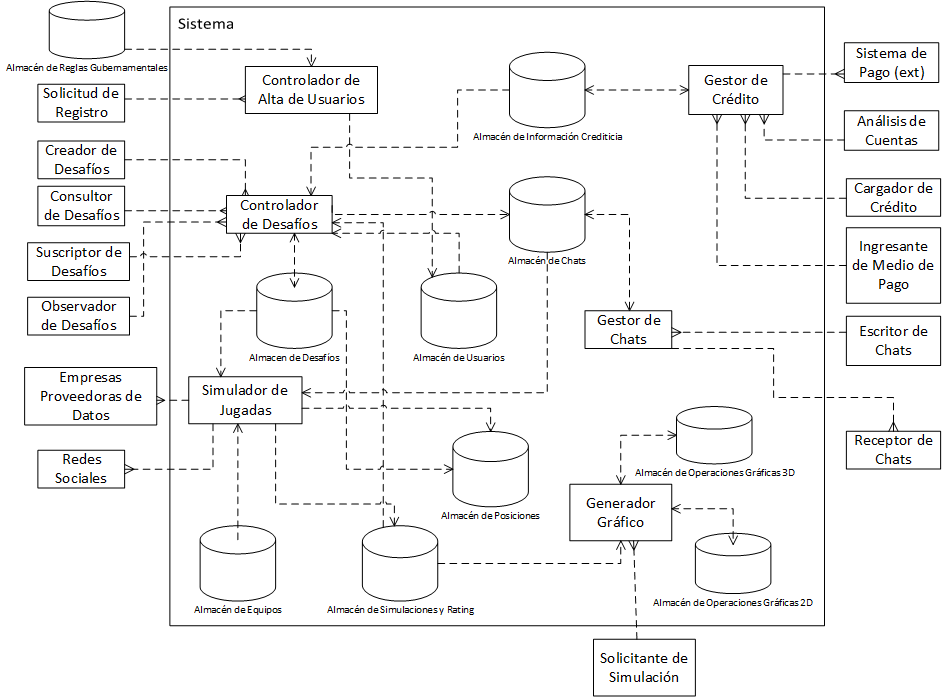
\includegraphics[scale=0.80,angle=90]{diagramas/arquitectura_general}
\label{fig:arquitectura_general}

En la figura \ref{fig:arquitectura_general} se ven los principales componentes del sistema, sobre los cuales se hace zoom en las secciones posteriores, además de los repositorios utilizados para nuestra solución.

\subsection{Controlador de Alta de Usuarios}
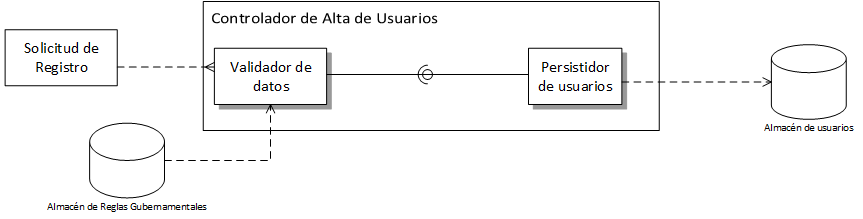
\includegraphics[scale=0.65]{diagramas/controlador_de_usuarios}
\label{fig:controlador_de_usuarios}

Toda \textbf{solicitud de registro} al sistema es recibida por el componente \emph{Controlador de Alta de Usuario}, que consta de tres etapas. 

El \emph{Validador de Datos} es la primera. Tal componente se encarga de validar las distintas posibilidades del usuario con respecto a las reglas gubernamentales establecidas en su país (que se consultan en el repositorio correspondiente). Es, básicamente, un filtro que le permite o no al usuario registrarse de acuerdo a la legislación vigente del territorio desde donde esté entrando al sistema.

Una vez validados los datos, si el usuario incluyó en su registro un método de pago, el \emph{Controlador de Alta de Medios de Pago} validará la información relativa al mismo con el servicio externo correspondiente, y la almacenará en el repositorio adecuado en caso de que sea correcta. El zoom de este componente se verá en la figura \ref{fig:gestor_de_credito}.

Por último, la tercer etapa, el \emph{Persistidor de Usuarios}, es el encargado, ya con todos los datos anteriores validados, de almacenarlos en el repositorio \emph{Almacén de Usuarios}, efectivizando así el registro del usuario.

\newpage
\subsection{Gestor de Crédito}
\begin{center}
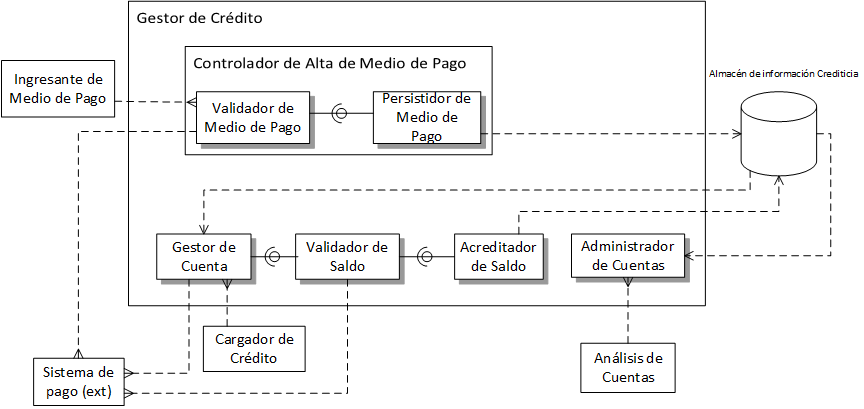
\includegraphics[scale=0.80,angle=90]{diagramas/gestor_de_credito}
\label{fig:gestor_de_credito}
\end{center}

Si un usuario desea pasar del servicio de modalidad gratuita (p.ej., en caso de no haber ingresado un medio de pago a la hora de registrarse) de nuestro sistema al servicio pago, puede realizarlo en cualquier momento (\emph{Ingresante de Medio de Pago}. El componente \emph{Controlador de Alta de Medio de Pago} es el encargado de recibir tales solicitudes, que siempre se encuentran encriptadas.

Este componente cuenta de dos pasos. El primero, \emph{Validador de Medio de Pago}, se encarga de validar la información ingresada comunicándose con el correspondiente servicio de medio de pago externo. El segundo, \emph{Persistidor de Medio de Pago}, es quien -una vez todas las validaciones hayan sido corroboradas y aceptadas- persiste esta información en el \emph{Almacén de Información Crediticia}.

Un usuario puede cargar crédito a su cuenta en cualquier momento (\emph{Cargador de Crédito}). Esta información llega al componente de manera encriptada, y deberá pasar por un pipeline de validaciones, que comienza en el \emph{Gestor de Cuenta}. Este primer paso consta de obtener todos los datos correspondientes a la cuenta, y validar que todavía esté activa. Una vez esta información haya sido confirmada por el \emph{Sistema de Pago (externo)}, el validador de saldo será el encargado de corroborar que la cifra a cargar en cuestión, tenga un respaldo en saldo en el edio de pago del usuario (consultando, nuevamente, al \emph{Sistema de Pago (externo)}). Si se confirma esto, el \emph{Acreditador de Saldo} será el que se comunique con el repositorio \emph{Almacén de Información Crediticia} e ingrese el nuevo saldo del usuario.

Cuando un usuario administrador desee consultar los datos de alguna cuenta (\emph{Análisis de Cuentas}), lo hará a través de un componente con privilegios especiales, el \emph{Administrador de Cuenta}, que tiene la capacidad de mostrar y analizar la información crediticia de todos los usuarios. Las comunicaciones con este componente se encuentran también cifradas.

\newpage
\subsection{Gestor de Chats}
\begin{center}
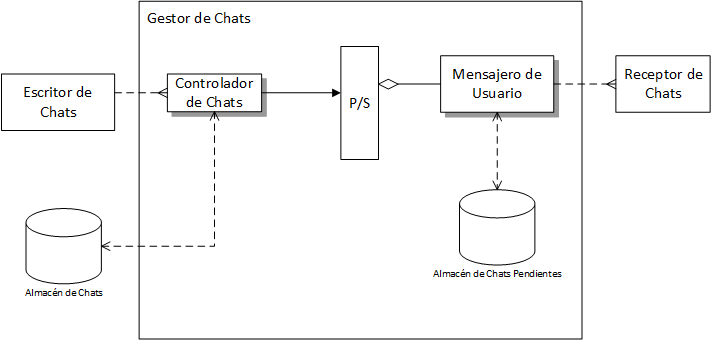
\includegraphics[scale=0.80]{diagramas/gestor_de_chats}
\label{fig:gestor_de_chats}
\end{center}

Los usuarios pueden escribir chats (\emph{Escritor de Chats}) o bien ser quien los recibe (\emph{Receptor de Chats}). Esto ocurre en los distintos tipos de chats que ofrece el sistema, tanto el global del desafío como el individual. 

Quien desee escribirle a otro usuario, se comunicará con el \emph{Controlador de Chats}, quien validará que la persona está disponible para comunicarse en ese chat global en el caso de que sea un chat de desafío, o creará/buscará un chat con el nuevo participante en el caso de los chats individuales. Una vez validada esta información, el componente publicará mediante uno conector del tipo \textbf{Publish/Subscribe} la nueva información de chat, y será alguno de los \emph{Mensajero de Usuario} quien se encargará de ponerlo a disponibilidad del receptor. 

Si el usuario receptor no está conectado para recibir el mensaje, el \emph{Mensajero de usuario} cuenta con su propio repositorio (\emph{Almacén de Mensajes Pendientes}, lo que le permite mantener control sobre los mensajes que aún le restan enviar.

\newpage
\subsection{Controlador de Desafíos}
\begin{center}
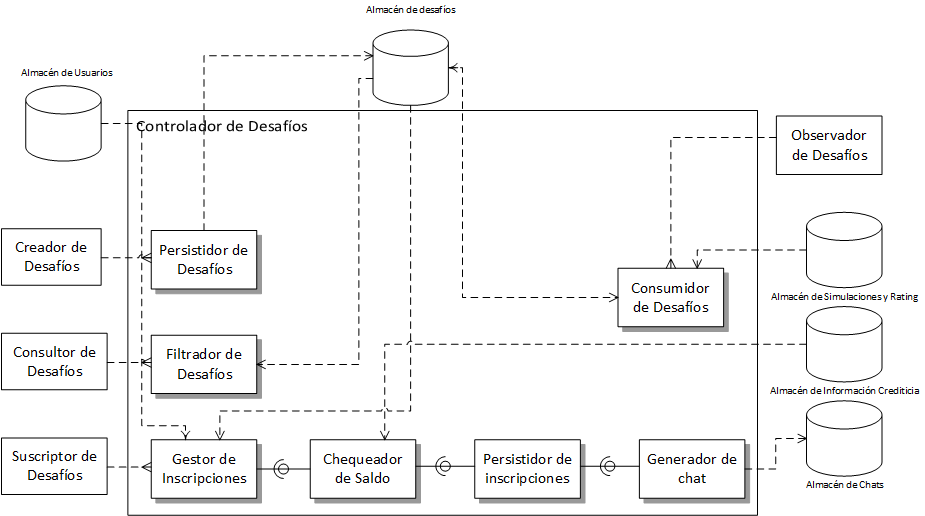
\includegraphics[scale=0.80,angle=90]{diagramas/controlador_de_desafios}
\label{fig:controlador_de_desafios}
\end{center}

El \emph{Controlador de Desafíos} es ya un componente más complejo que el anterior, y ofrece diversas interacciones.

Por un lado, el \emph{Creador de Desafíos} se comunica con el \emph{Persistidor de Desafíos} y le comunica sus intenciones de crear un nuevo desafío; el \emph{Persistidor} almacena el nuevo desafío en el \emph{Almacén de Desafíos}, desde donde puede ser consultado por otros de los componentes.

Cuando un usuario desea consultar los desafíos a los que puede inscribirse (\emph{Consultor de Desafíos}), el \emph{Filtro de Desafíos} se encarga de interactuar con los datos del usuario y el \emph{Almacén de Desafíos}, para presentar la información solicitada de manera correcta.

Cuando un usuario desea inscribirse en un desafío (\emph{Suscriptor de Desafíos}), el \emph{Gestor de Inscripciones} es quien recibe la petición con todos los datos del usuario y el desafío en cuestión, y analiza si es posible o no cumplir con el pedido. Si lo es, se le transmite la información al \emph{Chequeador de Saldo}, quien validará -en caso de ser necesario- que el usuario cuente con el saldo suficiente para participar del desafío. 
Estos datos, luego, pasan por un pipe al componente siguiente, quien es el encargado de persistir la información del registro del usuario en el desafío elegido, dejando constancia de la inscripción.
Finalmente, el \emph{Generador de Chat} es quien inscribe al nuevo usuario en el chat global del desafío.

Por otro lado, las noticias y comunicaciones relativas a los desafíos, estén dirigidas a usuarios inscriptos o no, son leídas por el \emph{Consumidor de Desafíos}, quien es el encargado de, a partir de los datos de los desafíos generados y las simulaciones, ofrecer la información correspondiente a quien sigue un desafío (\emph{Seguidor de Desafíos}).


\newpage
\subsection{Simulador de Jugadas}
\begin{center}
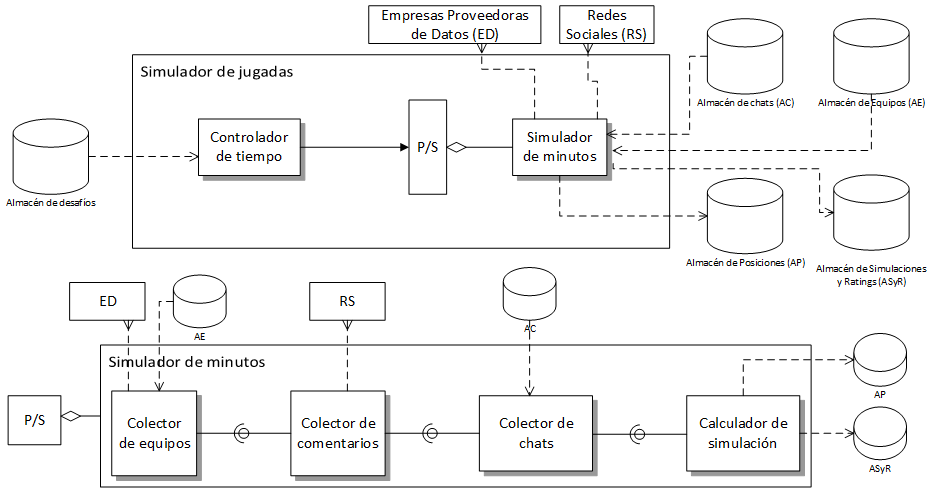
\includegraphics[scale=0.90,angle=90]{diagramas/simulador_de_jugadas}
\label{fig:simulador_de_jugadas}
\end{center}
\newpage
Cada vez que se le dé inicio a un desafío, es el \emph{Controlador de tiempo} del \emph{Simulador de Jugadas} el encargado de publicar la información en un conector de tipo \textbf{Publish/Subscribe}. El \emph{Simulador de Minutos} será quien realice todos los cálculos de la simulación, y los dejará disponibles en el repositorio correspondiente (\emph{Almacén de Simulaciones y Ratings}).

Realizando \emph{zoom} sobre el \emph{Simulador de Minutos}, vemos que se descompone de la siguiente manera:
\begin{itemize}
 \item \emph{Colector de Equipos}: este componente es el encargado de conectarse al \emph{Repositorio de Equipos} y traer la información necesaria de cada uno de los equipos que serán utilizados en la simulación del desafío. La información obtenida es entregada al siguiente componente, el
 \item \emph{Colector de Comentarios}: este componente recorre las distintas redes sociales de forma paralela con el objetivo de procesar la mayor cantidad de comentarios sobre los jugadores de las últimas horas para influir sobre el resultado de la simulación. Obtenida esta información (\textbf{\underline{Nota}}: asumimos que todas las redes sociales cuentan con algún servicio que pueda responder con baja latencia a búsquedas del tipo \'Lioner Messi\'), se enviará por medio de un pipe al siguiente componente en el camino, el
 \item \emph{Colector de Chats}: este componente/conjunto de componentes en paralelo se conecta con el repositorio \emph{Almacén de Chats} para buscar información y comentarios sobre los jugadores, técnicos, etc. de cada uno de los equipos del desafío. Recabada esta información, pasa al siguiente componente,
 \item \emph{Calculador de Simulación}: cuando llegue la información a este componente, la simulación será calculada y persistida en el \emph{Almacén de Simulaciones y Ratings}, junto al desempeño de cada uno de los jugadores participantes en el desafío y, en caso de estar calculando la última jugada del partido, las nuevas posiciones de los participantes en cuestión (persistidas en el \emph{Almacén de Posiciones}).
\end{itemize}


\newpage
\subsection{Generador Gráfico}
\begin{center}
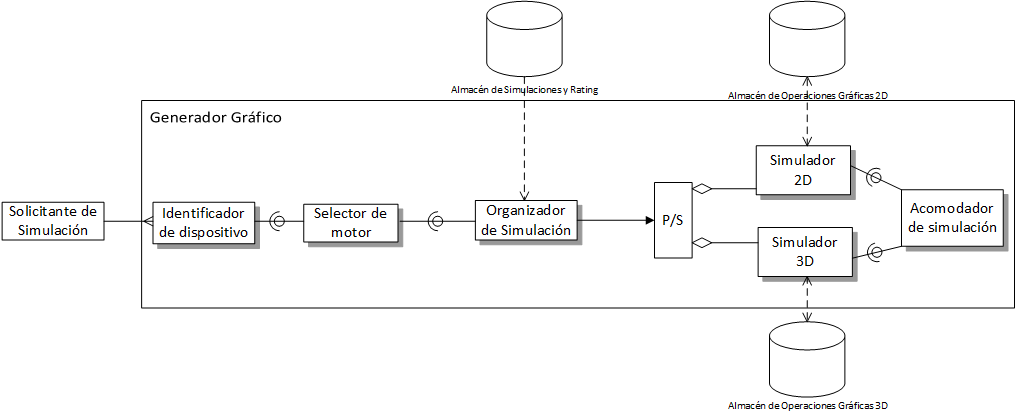
\includegraphics[scale=0.86,angle=90]{diagramas/generador_grafico}
\label{fig:generador_grafico}
\end{center}

Cuando un usuario solicite ver una simulación, será el \emph{Identificador de Dispositivo} el primero en recibir este pedido, y analizar las capacidades gráficas con las que cuenta el aparato en cuestión.

Esta información es enviada al \emph{Selector de Motor}, quien toma la decisión sobre qué motor es el más adecuado (si es que hay uno) para el dispositivo que realizó la solicitud, y envía el resultado mediante un pipe al \emph{Organizador de Simulación}.

Este componente es el encargado de buscar todos los datos necesarios en el repositorio \emph{Almacén de Simulaciones y Ratings}, y publicarlos con un conector Publish/Subscribe junto a la información del motor necesario.

Según el tipo de motor elegido (2D, 3D), el componente adecuado (\emph{Simulador \{2D,3D\}}) lee esa información del Publish/Subscribe, y es el encargado de calcular a partir de los datos recopilados, las instrucciones que reciben los motores gráficos de los dispositivos. Este componente consulta a su propio repositorio (\emph{Almacén de Operaciones Gráficas \{2D,3D\}}), con el fin de tener un caché de aquellos cálculos que se realizan de forma más frecuente. En el caso de que no sea posible utilizar el motor gráfico del dispositivo, un \emph{Motor 3D} en nuestros servidores recibe directamente las instrucciones para la simulación, la genera y la envía al \emph{Streamer}.

Una vez que las instrucciones para los motores (2D, 3D) de la simulación gráfica fueron generadas, este stream de datos que se calcula en tiempo real, será enviado a un último componente, el \emph{Acomodador de Simulación}. La función del mismo es enviar el stream como una serie de paquetes ordenados al dispositivo (de forma parecida al protocolo de sliding window en las conexiones TCP de Internet).


\newpage
\subsection{Streamer}
\begin{center}
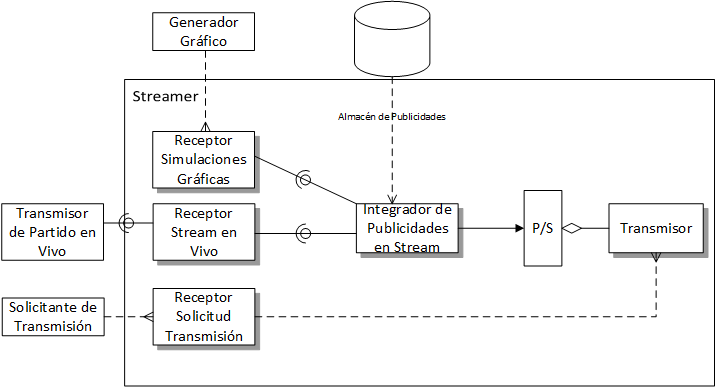
\includegraphics[scale=0.86,angle=90]{diagramas/streamer}
\label{fig:streamer}
\end{center}

El componente \emph{Streamer} es el encargado de realizar la transmisión de video hacia los dispositivos de los usuarios en dos casos, cuando los motores gráficos no soportan al dispositivo en cuestión, o cuando el usuario decidió ver la transmisión de un partido en vivo.

El usuario (\emph{Solicitante de Transmisión}) se comunica con el sistema cuando desea ver un partido en vivo antes de que empiece, y su pedido es recibido por el \emph{Receptor Solicitud de Transmisión}, quien lo reenvía al \emph{Transmisor}. Éste se subscribe al conector \emph{Publish/Subscribe} con el tipo de evento solicitado por el usuario, y queda a la espera de que sea transmitido.

Cuando alguna empresa con los derechos de transmisión de algún partido (\emph{Transmisor de Partido en Vivo}) desea ofrecerlo en nuestra plataforma, se comunica con nuestro sistema y el pedido es recibido por el \emph{Receptor de Stream en Vivo}. El receptor encola este stream en el \emph{Integrador de Publicidades en Stream}. 

Este componente agrega a las transmisiones (ya sean en vivo o simulaciones) las publicidades que se encuentren activas en el repositorio \emph{Almacén de Publicidades}. Luego, se conecta mediante el conector \textbf{Publish/Subscribe} al \emph{Transmisor}, al que le deja disponible el partido con publicidades 
integradas y listo para transmistir al \emph{Solicitante de Transmisión}.

En caso de las simulaciones que no pueden ser generadas en un dispositivo, llega el pedido desde el \emph{Generador Gráfico} al \emph{Receptor de Simulaciones Gráficas}, que encola también el video listo para transmitir en el \emph{Integrador de Publicidades en Stream}.

